\def\ZN{\mathbb{Z}_{N}}
\newcommand\qubit[1]{\left| #1 \right>}
\chapter{Алгоритм Шора для факторизации}
\section{Введение}

Есть число $N$
\begin{equation*}
  N = a \cdot b,\qquad a \neq b
\end{equation*}

\textbf{Задача факторизации}: для числа
$N = p_{1}^{\alpha_{1}} \cdots p_{t}^{\alpha_{t}}$
\begin{itemize}
  \item либо получить каноническую форму
  \item либо получить нетривиальный делитель
\end{itemize}

Число $a \in \mathbb{Z}_{N}$ \textbf{принадлежит показателю} $\delta$, если
$\delta$ --- минимальное число, для которого
$a^{\delta} \equiv 1 \mod n$.
Обозначаем $\delta_{N}\left( a \right)$.

Показатель существует только если $a$ и $N$ взаимно просты ($a \in \ZN$)
и по сути является порядком $a$ в группе
$\ZN: \delta_{n}\left( a \right) = ord_{N}\left( a \right)$.
Если $gcd\left( a, N \right) \neq 1$, то мы нашли нетривиальный делитель.

Допустим, что для заданного $a \in \ZN$ у нас есть оракул $O_{f}$,
который возвращает показатель числа.
Если этот оракул полиномиален, то можно факторизовать число (вероятностно)

Пусть $r$ --- чётное и $gcd\left( a^{r/2} + 1, N \right) = 1$,
где $O_{f}\left( a \right) = r$
\begin{equation*}
  \begin{split}
    a^{r} \ge 1 \mod N \\
    \left( a^{r/2} - 1 \right) \cdot \left( a^{r/2} + 1 \right) \equiv
      0 \mod N
  \end{split}
\end{equation*}
Но $a^{r/2} \neq 1 \mod N$, потому что иначе $r$ --- не минимальное число
(нарушение определения показателя).
Значит, $\left( a^{r/2} - 1 \right)$ и $N$ имеет нетривиальный общий делитель.

Важно: условие $gcd\left( a^{r/2} + 1, N \right) = 1$ можно заменить на
условие $a^{r/2} + 1 \nmid N$.

\begin{affirmation}
  Пусть $N = p_{1}^{\alpha_{1}} \cdots p_{t}^{\alpha_{t}}$ и
  \begin{equation*}
    S = \left\{ a \in \ZN: ord\left( a \right) mod 2 = 0
    \lor a^{ord\left( a \right)/2} + 1 \nmid N \right\}
  \end{equation*}
  Тогда
  \begin{equation*}
    \left| S \right| \le \frac{\varphi\left( N \right)}{2^k}
  \end{equation*}
\end{affirmation}

То есть, подходящих нам $a$ очень мало.

\section{Алгоритм факторизации с оракулом}

\begin{enumerate}
  \item Генерируем такое $a$, чтобы при $r = O_{f}\left( a \right)$ выполняось
    \begin{equation*}
      r = 2 \cdot r_1, a^{r_{\alpha}} + 1 \nmid N
    \end{equation*}
  \item $gcd\left( a^{r_1} - 1, N \right)$ --- нетривиальный делитель.
\end{enumerate}

\begin{affirmation}
  В классической модели найти оракул $O_f$ не получилось.
  Шору удалось построить его в квантовой модели.
\end{affirmation}

Рассмотрим функцию $f: \ZN \rightarrow \ZN$
\begin{equation*}
  f\left( x \right) = a^{x} \mod N
\end{equation*}
Это почти непериодическая функция --- её период не кратен $N$.

\section{Квантовая система}

У нас есть $\qubit{0}$, $\qubit{1}$; кубит находится в
суперпозиции состояний
$\alpha_1 \cdot \qubit{0} + \alpha_2 \qubit{1}$, над которыми
можно выполнять унитарные операции в пространстве Гильберта
$C \cdot \mathbb{Z}_2$.

Коэффициенты $\alpha_1, \alpha_2$:
\begin{itemize}
  \item
    $\alpha_1, \alpha_2 \in \mathbb{C}$,
  \item
    $\left| \alpha_1 \right|^2 + \left| \alpha_2 \right|^2 = 1$,
  \item
    $\left| \alpha_1 \right|^2$ --- вероятность попасть в $\qubit{0}$,
  \item
    $\left| \alpha_2 \right|^2$ --- вероятность попасть в $\qubit{1}$.
\end{itemize}

\begin{figure}[h!]
  \centering
    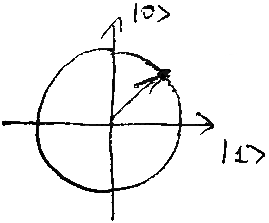
\includegraphics{qubit}
  \caption{Состояние кубита}
\end{figure}

К кубитам можно применять преобразование Уолша-Адамара
\begin{equation*}
  \begin{split}
    W\left( \qubit{0} \right)
      &= \frac{1}{\sqrt{2}} \cdot \left( \qubit{0} + \qubit{1} \right) \\
    W\left( \qubit{1} \right)
      &= \frac{1}{\sqrt{2}} \cdot \left( \qubit{0} - \qubit{1} \right) \\
  \end{split}
\end{equation*}

Набор кубитов --- одна из возможных интерпретаций квантово-механической системы.
Другой вариант --- $N$-уровневая система, в которое есть $N$ состояний
$\qubit{0}$, $\qubit{1}$, $\dots$, $\qubit{N-1}$, и
эти состояния ортонормированы (то есть, при измерении выпадают только эти
состояния и ничего среднего между ними).

\begin{figure}[h!]
  \centering
    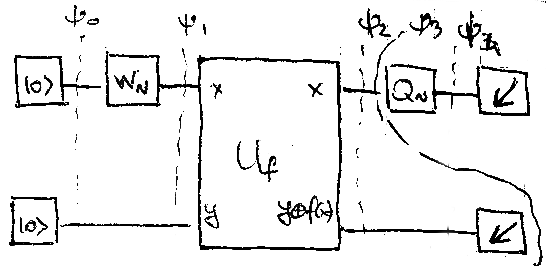
\includegraphics{shor}
  \caption{Алгоритм Шора}
  \label{fig:shor}
\end{figure}

Обозначения на рис. \ref{fig:shor}:
\begin{itemize}
  \item $\psi_i$ --- состояние системы,
  \item $W_N$ --- преобразование Уолша (или преобразование Фурье),
  \item $U_f$ --- стандартный оракул (базисный в квантовой модели),
  \item $Q_N$ --- преобразование Фурье,
  \item стрелочка --- измерение.
\end{itemize}

Что происходит?
\begin{enumerate}
  \item
    \begin{equation*}
      \qubit{\psi_0} = \qubit{0} \qubit{0}
    \end{equation*}
  \item 
    \begin{equation*}
      \qubit{\psi_1} = W_N\left( \qubit{0} \right) \otimes \qubit{0}
    \end{equation*}
    Свойство: $W_N\left( \qubit{0} \right)$ даёт равномерную суперпозицию
    (что Уолш, что Фурье), то есть
    \begin{equation*}
      W_N\left( \qubit{0} \right)
      = \frac{1}{\sqrt{N}}
        \cdot \left( \qubit{0} + \qubit{1} + \dots + \qubit{N-1} \right)
    \end{equation*}
  \item 
    Суперпозиция всех значений функции $f\left( x \right) = a^x \mod N$
    \begin{equation*}
      \qubit{\psi_2} = \frac{1}{\sqrt{N}} \cdot \left( \qubit{0} \cdot \qubit{a^0 \mod N} + \qubit{1} \cdot \qubit{a^1 \mod N} + \dots + \qubit{N-1} \cdot \qubit{a^{N-1}} \mod N \right)
    \end{equation*}
  \item Мы измерили второй регистр -- там второй кубит принял некоторое значение
    $\qubit{y_0}$
    \begin{equation*}
      \qubit{\psi_0} = \frac{1}{\sqrt{k}} \cdot \left( \qubit{x_0} + \qubit{x_0 + r} + \dots + \qubit{x_0 + \left( k-1 \right) \cdot r} \right) \cdot \qubit{y_0},
    \end{equation*}
    где $\qubit{x_0}$ --- все состояния $\qubit{x}$, для которых $f\left( x \right) = y_0$, $k = \lfloor \frac{N}{r} \rfloor$.
  \item Преобразование Фурье
    \begin{equation*}
      Q_N\left( \qubit{k} \right) = \frac{1}{\sqrt{N}} \cdot \sum_{t} \exp{\frac{2 \cdot \pi \cdot i}{N} \cdot k \cdot t} \cdot \qubit{t}
    \end{equation*}
    Применяя его к первому регистру, получаем
    \begin{equation*}
      \qubit{\psi_4} = \sum_{S} c\left( S \right) \cdot \qubit{S} \cdot \qubit{y_0},
    \end{equation*}
    где
    \begin{equation*}
      c\left( S \right) =
      \begin{cases}
        \frac{\sqrt{N}}{r} &, S \equiv 0 \mod \frac{N}{r}, \\
        0 &, S \neq 0 \mod \frac{N}{r}. \\
      \end{cases}
    \end{equation*}
    Таким образом это будет или $0$, или равномерная суперпозиция.
  \item Измеряем первый регистр --- можем получить тоьлко те $S$, у которых
    $c\left( S \right) \neq 0$, т.е. состояния вида $\qubit{\beta \cdot \frac{N}{r}}$, где $\beta$ --- неизвестная константа.
\end{enumerate}

Таким образом мы знаем какое-то число $S$ такое, что
\begin{equation*}
  S = \beta \cdot \frac{N}{r}.
\end{equation*}
Если $gcd\left( S, N \right) = 1$ и $N \mid r$, то всё, но у нас
$N \nmid r$! Поэтому на самом деле
\begin{equation*}
  \frac{S}{N} = \frac{\beta}{r},
\end{equation*}
и мы строим рациональные приближения при помощи цепных дробей.

Итоговая сложность алгоритма Шора --- $O\left( \log^3 N \right)$.
